\chapter{Implementation}
\label{chap:implementation}
\myTop{In this chapter we describe how we implement the concepts described in \chapref{chap:design}.
This chapter is divided into three sections where the three main components of our system are described, namely \nameref{sec:pglib},  \nameref{sec:projGroupRoomImpl}, and \nameref{sec:manProjGrpImpl}.
The implementation details presented here are paramount for \chapref{chap:test} and \chapref{chap:evalProduct}.}%
From \secref{sec:architecture} we know that there are three components, which must be implemented by us -- the administration tool to manage project group, the project group, and the virtual group room. 
The administration tool is implemented as an admin tool, which, as described in \secref{par:admintool}, is a special Moodle plugin type. 

%Recall \secref{sub:interActivities} where we designed the concept of project groups.
In the implementation of the project group concept we are faced with two choices. 
It can be implemented as courses (see \secref{sub:courses}) by creating a new view for the course page. 
By doing so we solve the problem of both implementing project groups and the virtual group room.
This will make it possible to use activity modules, described in \secref{par:activitymodules}, in the virtual group room.
Another option is to make a local plugin, which, as described in \secref{par:localplugin}, gives us basic functionality such as database installation and the possibility to extend the built-in navigation block. 
With a local plugin we cannot use activity modules since they are too strongly connected to courses. 
Instead we can use \block{}s for the functionality. 
%We choose to implement the \detdeandrelaver{}s as blocks as described in \secref{sub:interActivities}.
We choose to make a local plugin.

The local plugin includes both the project group library and the virtual group room.


\section{Project Group Library}
\label{sec:pglib}
%The \viewroom[] is implemented in the file \moodlefile{/local/projectgroup/view.php} and  t
The project group library is implemented in the file \moodlefile{/local/projectgroup/lib- .php}. 
The library includes several other files. % such as various helper files and one for each of the other three peer-groups. 
One for each of our peer-groups and several helper files. 
Our contribution to the library is located in the library file itself. 
%The project group library is build up by several files and consist of several functions and classes.
%The library itself is created by our subgroup, but it includes a file from each of the other groups. 
%This following sections only explains the functionality implemented by our subgroup. 
The library consists of approximately $300$ lines of code, including comments and whitespace and excluding any included files. 
All the functionality in the library is auxiliary functionality for the entire system. 
%In the later sections we refer to several functions, which are all located in the library. 

The following sections explain how project groups are put into a \moodle{} context and how we ensure that users have the correct permissions.

\subsection{Overwrite Context}
In \secref{sub:contextsystem}  the context system of Moodle is described.
In this section the creation of a custom context is described. 

To be able to define capabilities for the project groups and have different blocks for different project group we need our own context.
We will create our own context level and class.
We call the context \cl{context\_projectgroup}. 

Moodle does not support extension of contexts through one of the more than 30 different plugin types available \cite{plugin}. 
There two parts of the problem, the first is to create a new context and the second is to load it properly. 
We create a new context by making a new class which is very similar to \cl{context\_course} class and by defining the context level of project groups as a constant. 
The class header and the constant definition can be seen in \coderef{codeprojectgroupcontext}. 
The constant is set to 55 and is chosen because that context level is unused and it is close to the course context level. 
We regard the project group contexts to be at the same level as course contexts. 
However, project groups does not have categories like courses does.

\begin{lstlisting}[style=phpCode, caption=\myCaption{The context\_projectgroup class header and constant definition}, label=codeprojectgroupcontext]
define ('CONTEXT_PROJECTGROUP',55);
class context_projectgroup extends context {
...
\end{lstlisting}

When a context is loaded in a Moodle page it is instantiated by \fu{get\_context\_instance}, which takes a context level and an instance id. 
The instance id can be a course id or similar depending on the context level -- in our case it is a project group id. 
This function calls a static method in the \cl{context\_helper} class which uses a private array to translate the context level into a class name.
The overall system definition in \chapref{chap:systemDef} retain us from changing the core code of Moodle. 
If this constraint were not enforced the array could simply be extended directly in the code.  
Since the array used is private we can not extend the context system by overriding the \cl{context\_helper} class. 
The newly created context is only used in pages created in this project and we can therefore create our own version of \fu{get\_context\_instance}. 
The new function can be seen in \coderef{codeprojectgroupcontextinstance}.
\begin{lstlisting}[style=phpCode, caption=\myCaption{The function to get projectgroup context}, label=codeprojectgroupcontextinstance]
function get_projectgroup_context_instance( $instance = 0, $strictness = IGNORE_MISSING) 
{ 
    return context_projectgroup::instance($instance, $strictness);
}
\end{lstlisting}
The \vari{instance} variable denotes a project group id.
The \vari{strictness} variable 

With the new context and the function to instantiate it we can now make per project group permissions and add blocks to specific project group pages. 
\FloatBarrier
\subsection{Ensuring Permissions}
\label{sec:projectgrouproommanagerights}
Permissions can generally be divided in two types; read and write. 
Read permissions gives you the ability to view the content of the virtual group room while write lets you change the content. 
If a user has write permission he must also have read permissions, otherwise he cannot see the page he attempts to edit. 
To ensure the user attempting to enter a virtual group room has permission to enter the function \fu{has\_projectgroup\_read\_permission} is used. 
%It checks if the user is a member of the group. 
It checks if the user is an administrator or is a member of the project group. 
The administrator check is necessary since an administrator should be able to see any project group even if he is not a member of the project group. 

The function \fu{has\_projectgroup\_write\_permission} checks that the user has write permissions and uses the read permission function to check that the user has read permission.
If he does not have read permission he should not be able to edit the virtual group room. 
In the current implementation the write permissions function does not make extra checks to permissions since the permission levels for read and write are equivalent.

Because the functions are separate it is possible to change them individually later.
%Making both function gives the ability to later change this.
An example is that an end users requires that supervisors should only have read permissions. Then the change will only be in one place. 
Both functions can be found in the project group library.


\FloatBarrier

In the implementation of the project group we are faced with several choices. 
Project groups can be implemented as courses by creating a new view for the course page.  
This will make it possible to use activity modules, described in \ref{par:activitymodules}, in the project group. 
Another approach is to make a local plugin, which gives us basic functionality, such as database installation. 
With a local plugin we cannot use activity modules since they are too related to courses. 
Instead we can use blocks for the functionality. 
The later approach is chosen. 

\section{Project Group Room}
In this section the actual implementation of the project group room, its custom blocks, how the context system is used to implement our own context to allow better administration of blocks and capabilities, and the navigation to the users project groups is described.
The section presents how the project groups work from the perspective of the user. 


\subsection{The page}
The project group page is the virtual meeting place described in \secref{sec:projectgroup}.
We decided to implement the room merely as a container for blocks. 
Alternatively the functionality could be an integrated part of the page, but using blocks gives more flexibility to the users allowing them manage the layout of their own project group room. 
A screenshot of a project group room can be seen in \figref{fig:projectgroupnoedit}. 
In this project group room the blocks are layouted as they are per default. 
\begin{figure}[h]
	\centering
		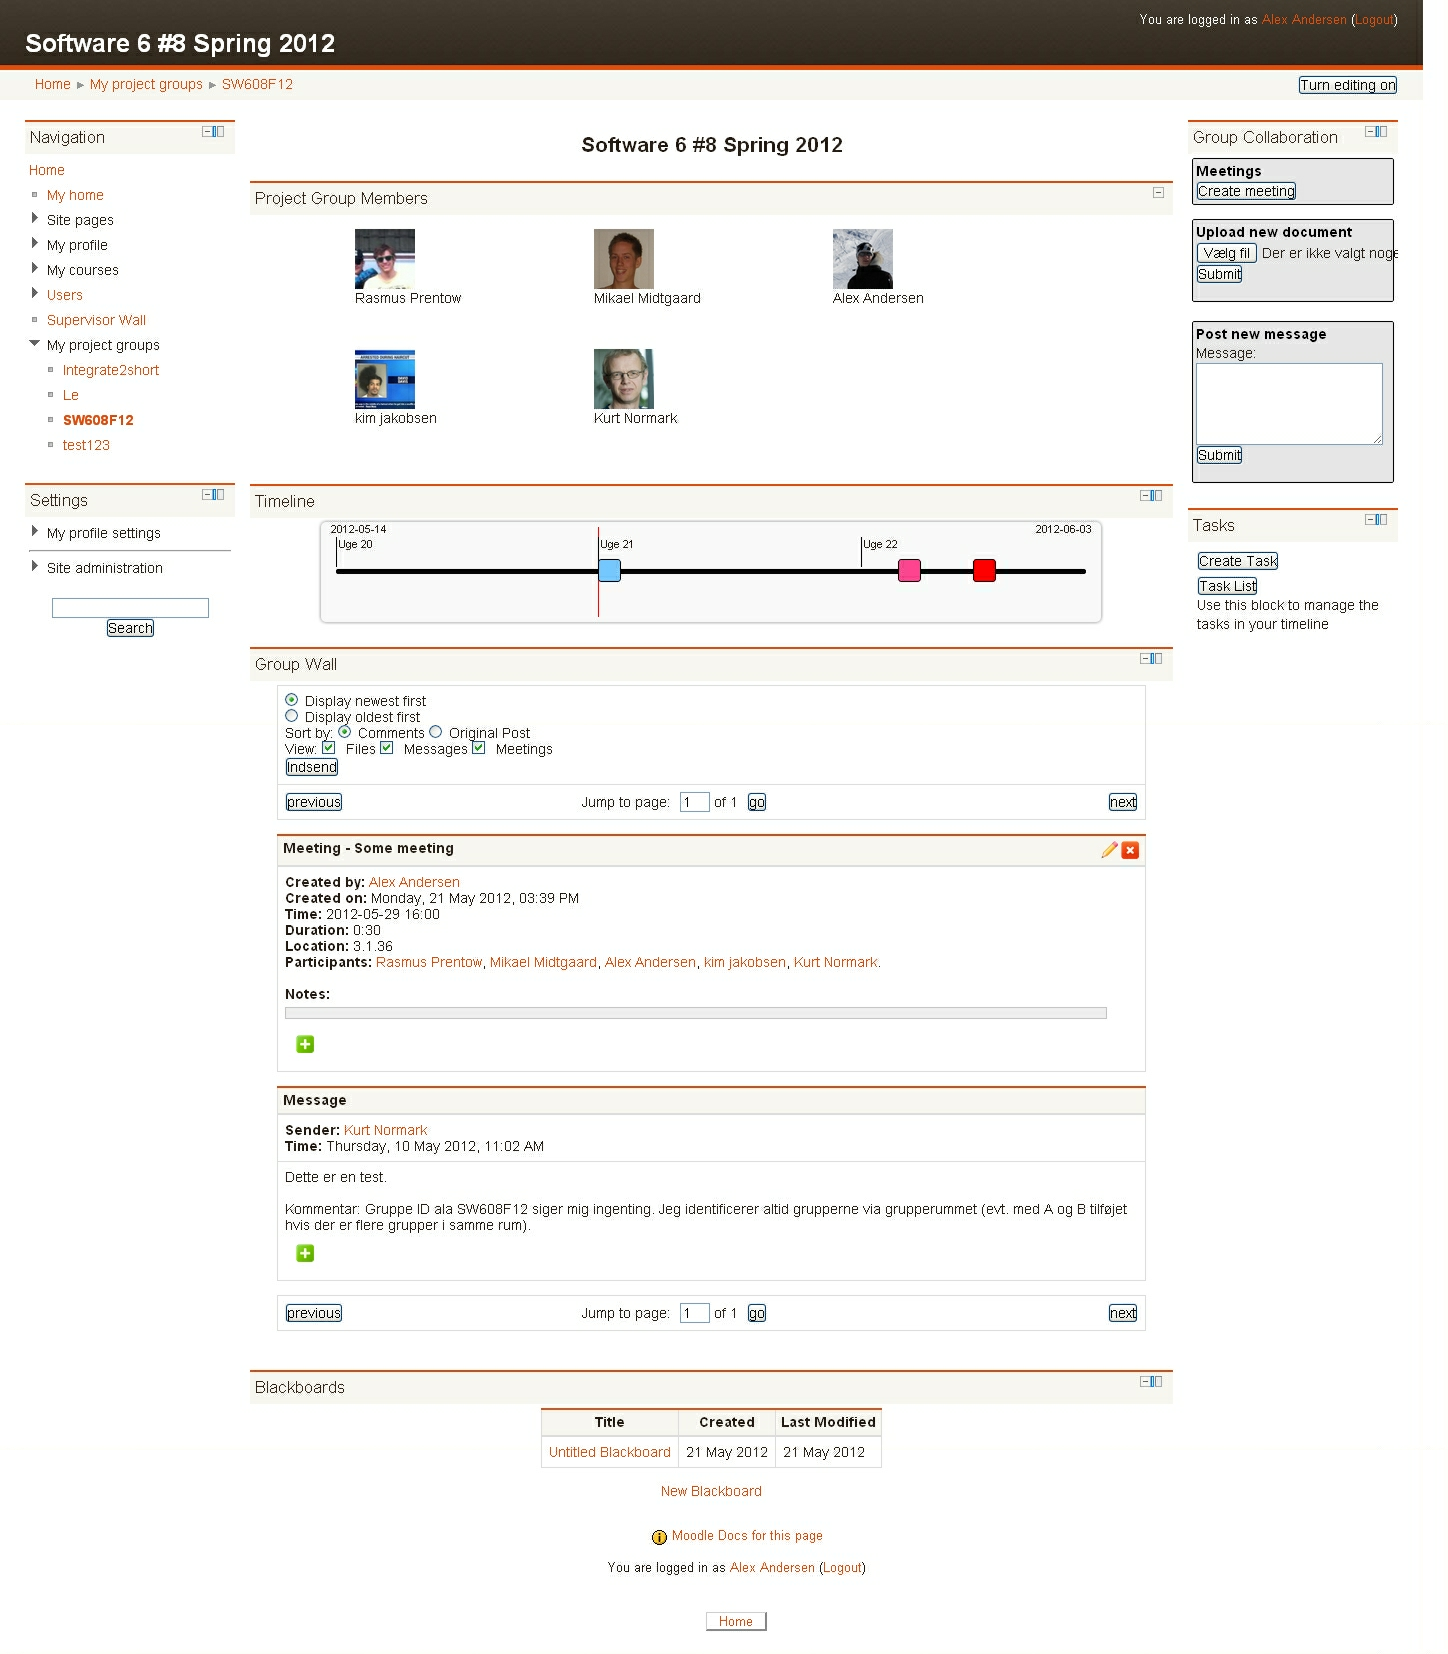
\includegraphics[width=\textwidth]{images/projectgroupnoedit.png}
	\morscaption{The project group room}
	\label{fig:projectgroupnoedit}
\end{figure}

The project group room consist of three columns. 
The left column is the standard navigation menu in Moodle. 
The Center and right columns both contain blocks.
The various blocks presented on the project groups page is described in \secref{sec:implprojectgroupblocks}. 
If an user wants to edit the block layout for the project group room he can press the ``Turn editing on'' button. 
This will add edit and move buttons to each block. 
A new block is added in editing mode to allow for adding new blocks. 
If an user edits the page the change can be seen by all group members. 
The page in edit mode can be seen in figure \figref{fig:projectgroupwithedit}.

\begin{figure}[h]
	\centering
		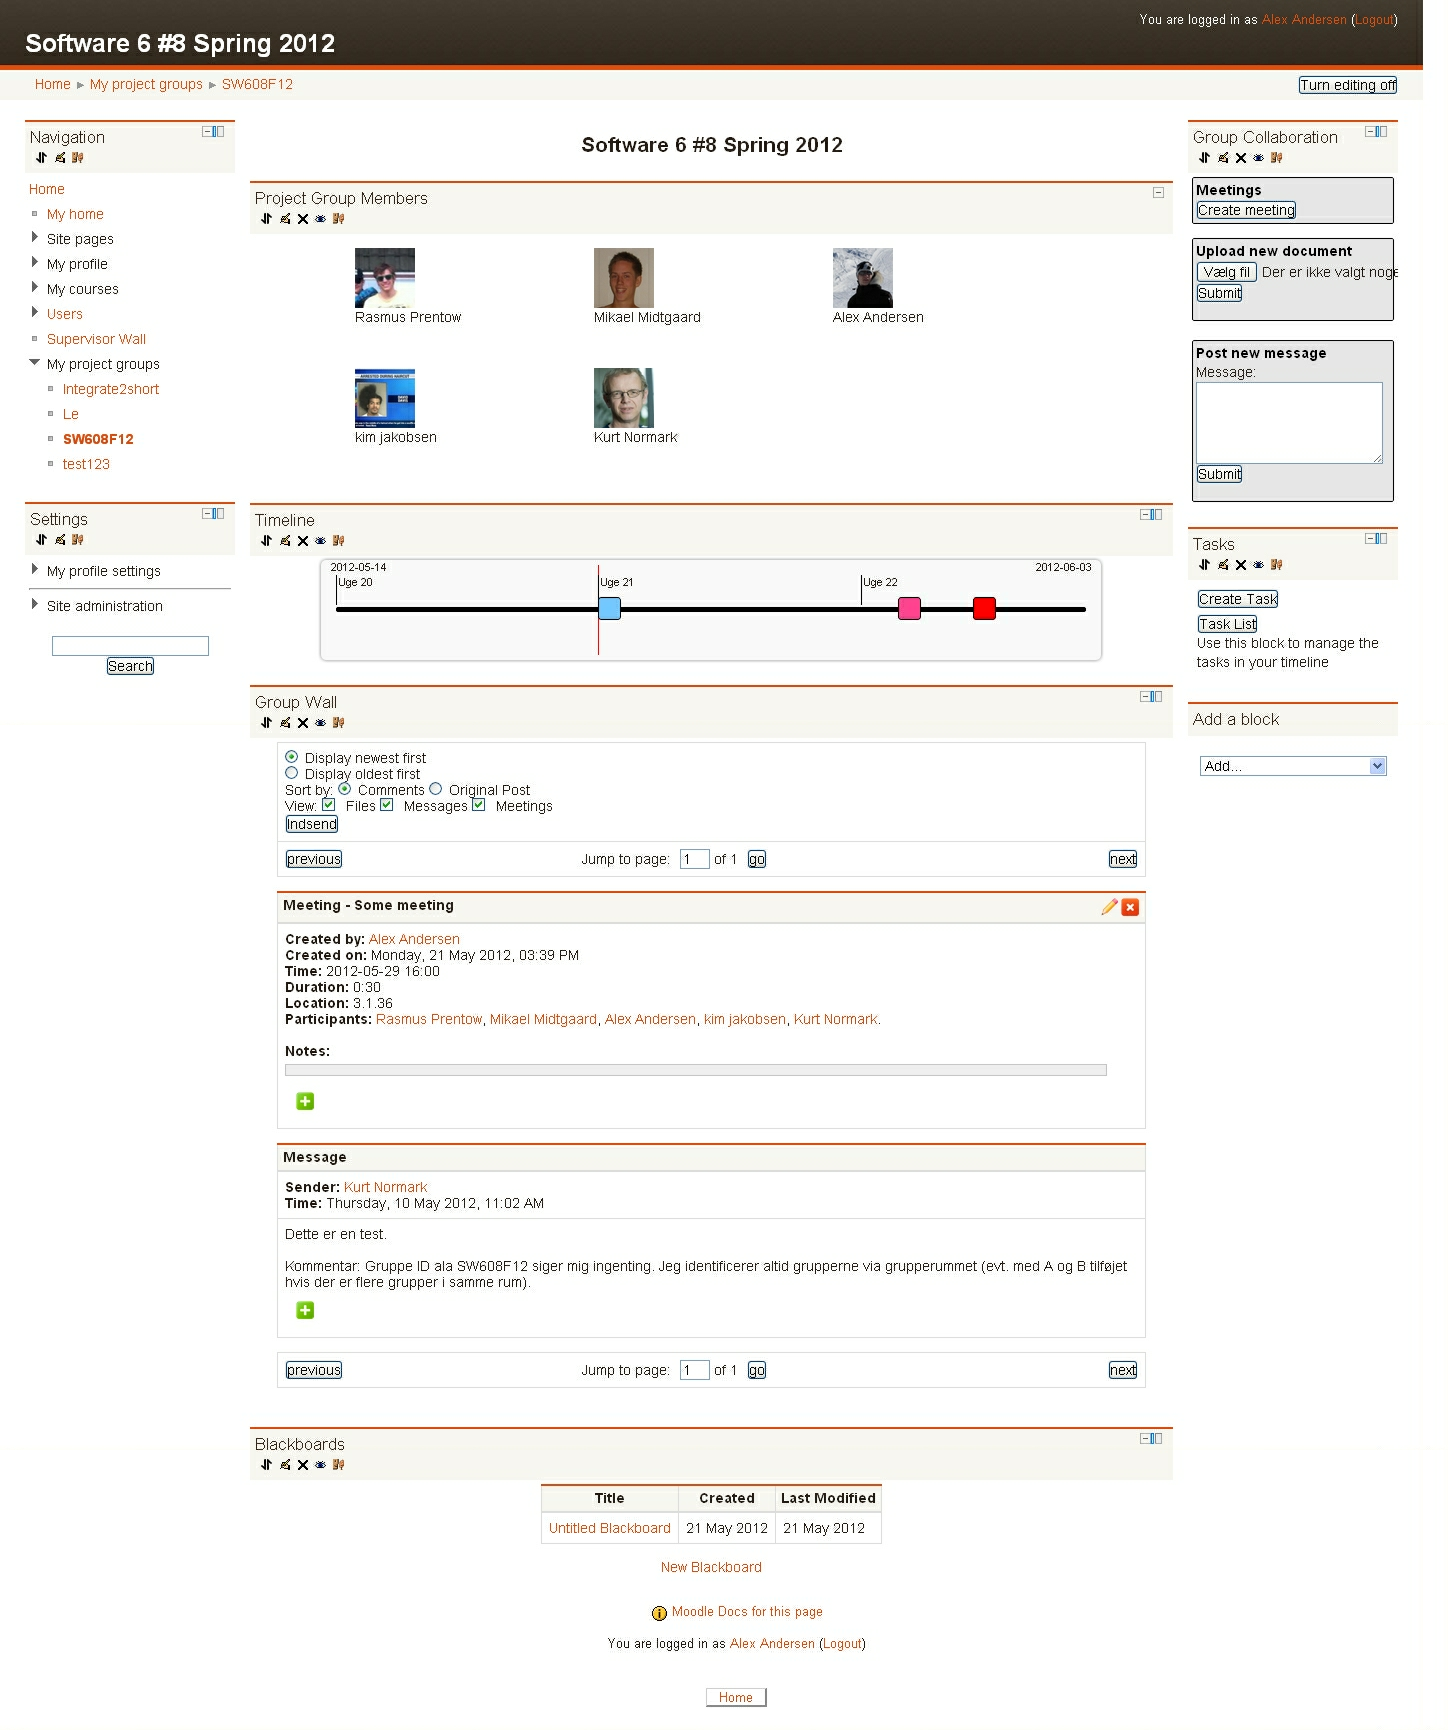
\includegraphics[width=\textwidth]{images/projectgroupwithedit.png}
	\morscaption{The project group room with editing turned on}
	\label{fig:projectgroupwithedit}
\end{figure}


The task of securing that only members of the project group can edit and view are maintained by the project group room and is described in \secref{sec:projectgrouproommanagerights}. 




\subsection{Ensuring Permissions}
\label{sec:projectgrouproommanagerights}
Permissions can generally be divided in two types; read and write. 
Read permissions gives you the ability to view the content of the project group room while write lets you change the content. 
If a user has write permission he must also have read permissions. 
Otherwise he cannot see the page he attempts to edit. 
To ensure the user attempting to enter a project group room has permission to enter the function \fu{has\_projectgroup\_read\_permission} is used. 
It checks if the user is an administrator or is a member of the group. 
The administrator check is necessary since administrators should be able to see the group even if they are not members of the group. 

The function  \fu{has\_projectgroup\_write\_permission} which checks that the user has write permissions uses the read permissions function too check that the user can read.
If he cannot read he should not be able to edit. 
In the current implementation the write permissions function does not make extra checks to permissions since the permission level for read and write is equivalent.
Making both function gives the ability to later change this.
An example could be if the potential users requires that their supervisor should only have read permissions. 
Then the change will be in one place only. 

\subsection{Blocks}
\label{sec:implprojectgroupblocks}
When a new project group is created the default blocks are added to the page. 
The default blocks are specified in the a config file and the content can be seen in \coderef{moodledaultblock}


\begin{lstlisting}[style=phpCode, caption=\myCaption{The default block configuration}, label=moodledaultblock]
<?php
	/**
	* Example usage:
	* "left1,left2:center1:right1"
	* Will add two items to the left, one in the middle, and one to the right
	*/
	$format['defaultprojectgroupblocks'] = ':projectgroup_members,timeline,groupwall,blackboard:upload,tasks';
\end{lstlisting}\begin{comment}$\end{comment}
The syntax for the format is $left:middle:right$. 
Left, middle, and right represent the three columns in the project group room. 
The blocks: Timeline, groupwall, blackboard, upload, and tasks is created by our peer-groups while the block named projectgroup\_members is created by us. 
The projectgroup\_members block shows the name and pictures of the project group members. 

	
	


\subsection{Overwrite Context}
In \secref{sub:contextsystem}  the context system of Moodle is described.
In this section the creation of a custom context is described. 

To be able to define capabilities for the project groups and have different blocks for different project group we need our own context.
We will create our own context level and class.
We call the context \cl{context\_projectgroup}. 

Moodle does not support extension of contexts through one of the more than 30 different plugin types available \cite{plugin}. 
There two parts of the problem, the first is to create a new context and the second is to load it properly. 
We create a new context by making a new class which is very similar to \cl{context\_course} class and by defining the context level of project groups as a constant. 
The class header and the constant definition can be seen in \coderef{codeprojectgroupcontext}. 
The constant is set to 55 and is chosen because that context level is unused and it is close to the course context level. 
We regard the project group contexts to be at the same level as course contexts. 
However, project groups does not have categories like courses does.

\begin{lstlisting}[style=phpCode, caption=\myCaption{The context\_projectgroup class header and constant definition}, label=codeprojectgroupcontext]
define ('CONTEXT_PROJECTGROUP',55);
class context_projectgroup extends context {
...
\end{lstlisting}

When a context is loaded in a Moodle page it is instantiated by \fu{get\_context\_instance}, which takes a context level and an instance id. 
The instance id can be a course id or similar depending on the context level -- in our case it is a project group id. 
This function calls a static method in the \cl{context\_helper} class which uses a private array to translate the context level into a class name.
The overall system definition in \chapref{chap:systemDef} retain us from changing the core code of Moodle. 
If this constraint were not enforced the array could simply be extended directly in the code.  
Since the array used is private we can not extend the context system by overriding the \cl{context\_helper} class. 
The newly created context is only used in pages created in this project and we can therefore create our own version of \fu{get\_context\_instance}. 
The new function can be seen in \coderef{codeprojectgroupcontextinstance}.
\begin{lstlisting}[style=phpCode, caption=\myCaption{The function to get projectgroup context}, label=codeprojectgroupcontextinstance]
function get_projectgroup_context_instance( $instance = 0, $strictness = IGNORE_MISSING) 
{ 
    return context_projectgroup::instance($instance, $strictness);
}
\end{lstlisting}
The \vari{instance} variable denotes a project group id.
The \vari{strictness} variable 

With the new context and the function to instantiate it we can now make per project group permissions and add blocks to specific project group pages. 



\subsection{Navigation}



























\section{Managing Project Groups} %Jeg skriver kun om admin funktionalitet her -Mikael ~♥
Before any project group can be useful it has to be created first.
Administrators need to have the ability to add, edit, and delete project groups.
The administration tools we provide have to be easy and fast to use, since they potentially have to be used many times.
This section describes how we implemented the administration tools needed to manage project groups.

The features we provide to manage project groups are known as administration tools in Moodle and can be accessed in the site administration menu as seen in \figref{fig:navigation}.

\begin{figure}[htb]
	\centering
		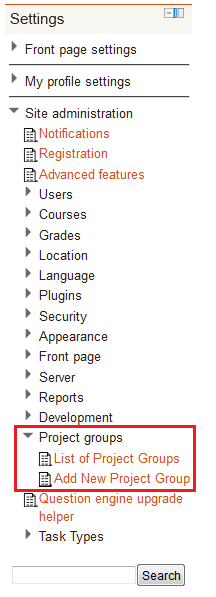
\includegraphics[scale=0.75]{images/admin-navigation.png}
	\morscaption{The settings block, which contains the site administration menu} 
	\label{fig:navigation}
\end{figure}

From here we provide a link to a list of all project groups and a link to a page, from where a new project group can be created.
The page with the list of all project groups has a table with three columns: Short name, Full name, and Actions.
As the name indicates Short name is a short name for a group. 
The Short name also serves as a link to the project group page described in \recref{sub:page}.
In the Actions column there are links to delete and edit the project group.

The edit page has the same source files as the add page.







